\documentclass[a4paper, 12pt, final, garamond]{book}
\usepackage{cours-preambule}

\raggedbottom

\makeatletter
\renewcommand{\@chapapp}{Architecture de la mati\`ere -- chapitres}
\renewcommand\thechapter{1 et 2}
\makeatother

\begin{document}
% \setcounter{chapter}{0}

\chapter{TD~: structures chimiques et propri\'et\'es macro}

% \makeatletter
% \renewcommand\thechapter{1 et 2}
% \makeatother

\section{Structures de \textsc{Lewis}}
\begin{enumerate}
    \item Donner le schéma de \textsc{Lewis} des espèces suivantes~:
        \[
            \ce{CH2Cl2}
            \qquad
            \ce{O2}
            \qquad
            \ce{C2H4}
            \qquad
            \ce{H3O+}
            \qquad
            \ce{HO-}
            \qquad
            \ce{H2CO}
            \qquad
            \ce{SiO2}
            \qquad
            \ce{CH3NH2}
        \]
    \item L'ozone \ce{O3} est une molécule non cyclique. Proposer une structure.
    \item \textit{Formule de \textsc{Lewis} de l'acide sulfurique}
    \begin{enumerate}[]
        \item Donner le schéma de \textsc{Lewis} de l'acide sulfurique
            \ce{H2SO4}. Dans cette molécule, les quatre atomes d'oxygène sont
            reliés à l'atome de soufre.
        \item En déduire celles des ions \ce{HSO4-} et \ce{SO4^{2-}}.
    \end{enumerate}
    \item Donner le schéma de \textsc{Lewis} des ions hydrogénocarbonate
        \ce{HCO3-} et carbonate \ce{CO3^{2-}}.
    \item Donner le schéma de \textsc{Lewis} du benzène \ce{C6H6}, qui est une
        molécule cyclique.
\end{enumerate}

\section{Le phosphore}
\begin{enumerate}
    \item Donner le nombre d'électrons de valence du phosphore \ce{P}.
    \item Donner la représentation de \textsc{Lewis} de la molécule \ce{PCl3}.
    \item Le phosphore peut aussi former \ce{PCl5}, pourquoi~? Préciser sa
        structure de \textsc{Lewis}.
\end{enumerate}

\section{Caractéristiques de quelques solvants}
On s'intéresse aux solvants suivants~:

\begin{table}[ht]
    \centerfloat
    % \caption{Caractéristiques de solvants.}
    \begin{threeparttable}
        \label{tab:solvtd}
        \begin{tabular}{p{3.5cm}ccccc}
            \toprule
            Nom &
            Eau &
            Méthanol &
            Hexane &
            DMF\tnote{1} &
            Acétonitrile
            \\\midrule
            Représentation &
            \cfig{\lewis{13,O}(-[5,.7]H)(-[7,.7]H)} &
            \cfig{CH_3-[,.7]\lewis{26,O}-[,.7]H} &
            \cfig{CH_3-{{(CH_2)}_4}-CH_3} &
            \cfig{N(-[3,.7]CH_3)(-[5,.7]CH_3)-[,.7]C(=[6,.7]\lewis{57,O})-[,.7]H} &
            \cfig{CH_3-[,.7]C~[,.7]\lewis{0,N}}
            \\[2.3em]\midrule\addlinespace
            Moment dipolaire &
            \SI{1.8}{D} &
            \SI{1.65}{D} &
            \SI{0}{D} &
            \SI{3.8}{D} &
            \SI{3.9}{D}
            \\\midrule
            \shortstack[l]{Permittivité\\ relative ($\ep_r$)} &
            \num{78.5} &
            \num{32.6} &
            \num{2.0} &
            \num{36.7} &
            \num{37.5}
            \\\bottomrule
        \end{tabular}
        \begin{tablenotes}[flushleft]
        \item[1] DMF est l'abréviation de diméthylformamide.
        \end{tablenotes}
    \end{threeparttable}
\end{table}

\begin{enumerate}
    \item Identifier les solvants polaires et apolaires.
    \item Identifier les solvants protiques et aprotiques.
    \item Identifier les solvants peu dispersifs, dispersifs, fortement
        dispersifs.
    \item Tous ces solvant sont miscibles entre eux, à l'exception de l'hexane.
        Expliquer pourquoi.
\end{enumerate}

\section{Températures de changements d'état}
On indique ci-après les valeurs de température d'ébullition de composés
apolaires~:

\begin{table}[ht]
    \centering
    \label{tab:tebapo}
    \begin{tabular}{lcccccc}
        \toprule
        Corps &
        \ce{H2} & \ce{N2} & \ce{O2} & \ce{F2} & \ce{Cl2} & \ce{Br2}
        \\\midrule
        $T_{\rm eb} (\si{K})$ &
        \num{20} & \num{77} & \num{90} & \num{85} & \num{238} & \num{331}
        \\\bottomrule
    \end{tabular}
\end{table}

\begin{enumerate}
    \item Interpréter l'évolution constatée.
\end{enumerate}
On indique ci-après les valeurs de température d'ébullition de composés
\textbf{polaires} de taille comparable~:
\begin{table}[H]
    \centering
    \label{tab:tebpo}
    \begin{tabular}{lcc}
        \toprule
        Composé & \ce{PH3} & \ce{H2S}
        \\\midrule
        Moment dipolaire (\si{D}) & \num{0.55} & \num{0.97}
        \\\midrule
        $T_{\rm eb} (\si{K})$ & \num{185} & \num{212}
        \\\bottomrule
    \end{tabular}
\end{table}
\begin{enumerate}[resume]
    \item Interpréter l'évolution constatée.
    \item Identifier les substances possédant la température de fusion la plus
        basse et la plus haute parmi la liste suivante~: hélium \ce{He}, argon
        \ce{Ar}, méthane \ce{CH4}, acide éthanoïque \ce{CH3COOH}. Justifier de
        manière précise et concise.
    \item Justifier la différence de température de fusion $T_{\rm fus}$ entre
        les deux molécules suivantes~:
\end{enumerate}
\begin{minipage}{0.49\linewidth}
    \begin{gather*}
        \cfig{C(-[3]Cl)(-[5]H)=C(-[1]Cl)(-[7]H)}
        \\
        \text{(Z)-1,2-dichloroéthène}
        \\
        T_{\rm fus} = \SI{342.1}{K}
    \end{gather*}
\end{minipage}
\hfill
\begin{minipage}{0.49\linewidth}
    \begin{gather*}
        \cfig{C(-[3]H)(-[5]Cl)=C(-[1]Cl)(-[7]H)}
        \\
        \text{(E)-1,2-dichloroéthène}
        \\
        T_{\rm fus} = \SI{321.7}{K}
    \end{gather*}
\end{minipage}

\section{Moment dipolaire et charges partielles}
\begin{enumerate}
    \item Pour la molécule \ce{HF}, le moment dipolaire vaut $p = \SI{1.83}{D}$,
        et la longueur de liaison est de \SI{92}{pm}. Calculer les charges
        partielles portées par chaque atome.
    \item Pour la molécule \ce{LiF}, la longueur de liaison vaut \SI{152}{pm}.
        La charge partielle positive est $\de = \num{0.9}\times e$. Calculer le
        moment dipolaire de cette molécule $p$ et préciser son orientation.
\end{enumerate}
\textit{Données}~: $e = \SI{1.6e-19}{C}$, et $\SI{1}{D} =
\frac{1}{3}\times\SI{e-29}{C.m}$

\section{Monoxyde de carbone}
La molécule de monoxyde de carbone est constituée d'un atome d'oxygène ($Z = 8$)
et d'un atome de carbone ($Z=6$). \bigbreak

\begin{enumerate}
    \item Donner le nombre d'électrons de valence des atomes d'oxygène et de
        carbone.
    \item Expliquer pourquoi le carbone est tétravalent (susceptible de former 4
        liaisons covalentes).
    \item Proposer une représentation de \textsc{Lewis} de monoxyde de carbone.
    \item La formule de \textsc{Lewis} proposée est-elle alors en accord avec
        les électronégativités du carbone et de l'oxygène~?
\end{enumerate}

\section{Températures d'ébullition}
Les températures d'ébullition sous \SI{1}{bar} des composés hydrogénés de la
14\ieme\ colonne et de la 17\ieme\ colonne du tableau périodique sont indiquées
sur le graphique ci-dessous~:

\begin{figure}[]
    \centering
    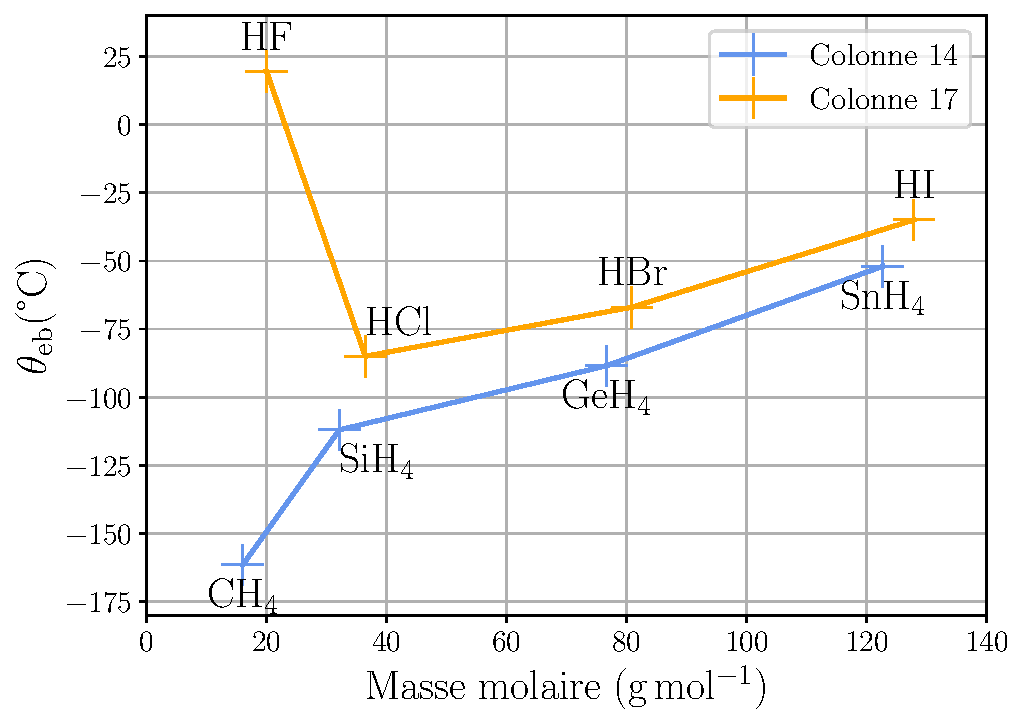
\includegraphics[scale=1]{teb_hydro}
    \label{fig:tebhydro}
\end{figure}

\begin{enumerate}
    \item La représentation de \textsc{Cram} de la molécule de méthane est
        représentée ci-dessous~:
        \begin{center}
            \cfig{C(-[2]H)(<:[5]H)(<[6]H)(-[7]H)}
        \end{center}
        \begin{enumerate}
            \item En déduire le moment dipolaire de la molécule de méthane.
            \item En déduire la géométrie et le moment dipolaire des autres
                composés hydrogénés de la colonne 14.
        \end{enumerate}
    \item Pourquoi les composés hydrogénés des éléments de la colonne 14 ont-ils
        des température d'ébullition plus basses que celles des composés
        hydrogénés de la colonne 17~?
    \item Expliquer l'augmentation observée entre \ce{HCl} et \ce{HI}.
    \item Proposer une explication à l'anomalie observée pour \ce{HF}.
\end{enumerate}

\end{document}
